\documentclass[12pt, a4paper, simple]{eskdtext}

\usepackage{hyperref}
\usepackage{_env/gpi_global.env}
\usepackage{_env/gpi_report.env}
\usepackage{_sty/gpi_lst}
\usepackage{_sty/gpi_toc}
\usepackage{_sty/gpi_t}
\usepackage{_sty/gpi_p}
\usepackage{_sty/gpi_u}

% Переменные
\def \gpiDocNum {2}
\def \gpiTopicRep {Размещение и оптимизация структуры элементов
автоматизированной системы обработки информации (АСОИ)}

% Код
% \ESKDletter{О}{Л}{Р}
% \def \gpiDocTypeNum {81}
% \def \gpiDocVer {00}
% \def \gpiCode {\ESKDtheLetterI\ESKDtheLetterII\ESKDtheLetterIII.\gpiStudentGroupName\gpiStudentGroupNum.\gpiStudentCard-0\gpiDocNum~\gpiDocTypeNum~\gpiDocVer}

\def \gpiDocTopic {Отчёт лабораторной работы №\gpiDocNum}

% колонтитулы
\usepackage{fancybox, fancyhdr}
\fancypagestyle{plain}
{
    \renewcommand{\footrulewidth}{0pt}          % Толщина отделяющей полоски снизу
    \renewcommand{\headrulewidth}{0pt}          % Толщина отделяющей полоски сверху
    \fancyhead[C]{ }                            % Коллонтитул сверху
    \fancyfoot[C]{\hfill\hfillстр. \thepage}    % Коллонтитул снизу
}

% Графа 1 (наименование изделия/документа)
% \ESKDcolumnI {\ESKDfontII \gpiTopic \\ \gpiDocTopic}

% Графа 2 (обозначение документа)
% \ESKDsignature {\gpiCode}

% Графа 9 (наименование или различительный индекс предприятия) задает команда
% \ESKDcolumnIX {\gpiDepartment}

% Графа 11 (фамилии лиц, подписывающих документ) задают команды
% \ESKDcolumnXIfI {\gpiStudentSurname}
% \ESKDcolumnXIfII {\gpiTeacherSurname}
% \ESKDcolumnXIfV {\gpiTeacherSurname}

\begin{document}
    \begin{ESKDtitlePage}
    \ESKDstyle{empty}
    \begin{center}
        \gpiMinEduRep \\
        \gpiEduRep \\
        \gpiKafRep \\
    \end{center}

    \vfill

    \begin{center}
        Тема: <<\gpiTopicRep>>
    \end{center}

    \vfill

    \begin{center}
        \textbf{\gpiDocTopic} \\
        по дисциплине \gpiDisciplineRep \\
    \end{center}

    \vfill

    \begin{flushright}
        \begin{minipage}[t]{7cm}
            Выполнил:\\
            \PageTitleStudentInfo
            \PageTitleDateField
            \hspace{0pt}

            Проверил:\\
            \PageTitleTeacherInfo
            \PageTitleDateField
        \end{minipage}
    \end{flushright}

    \vfill

    \begin{center}
        \PageTitleCity~\ESKDtheYear
    \end{center}
\end{ESKDtitlePage}

    \ESKDstyle{empty}
    \thispagestyle{plain}
    \pagestyle{plain}

    \begin{center}
        \textbf{\gpiDocTopic}
    \end{center}

    % = = = = = = = =
    \paragraph{} \textbf{Тема}: <<\gpiTopicRep>>

    \paragraph{} \textbf{Цель}:
    Формирование знаний и умений по размещению и оптимизации элементов АСОИ.

    \paragraph{} \textbf{Оптитмизация рабочих станций АСОИ}

    Оптимизация РС АСОИ включает решение следующих подзадач:
    
    \begin{enumerate}
        \item[1.] Формирование таблицы исходных данных для оптимизации количества РС АСОИ (см. табл.3.1).
        \item[2.] Оптимизация количества РС АСОИ.
        \item[3.] Формирование итоговых результатов оптимизации.
    \end{enumerate}

    \textbf{Формирование исходных данных}.
    Таблица для оптимизации (табл. 3.1) создается на основе информации из табл.В.1, табл.Г.1
    и решений принятых по ЭП (количество и режим сменности).

    Примеры таблиц приведены ниже.
    Для ЭП определено 4 сотрудника, которые обслуживают АСОИ в три смены (режим сменности равен три).

    \begin{figure}[h!]
        \centering
        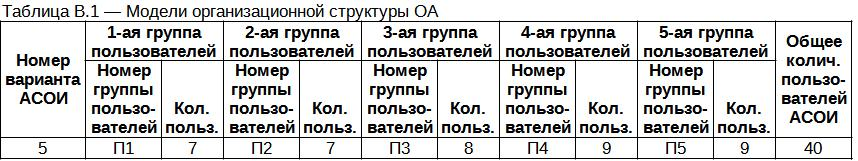
\includegraphics[width=14cm]
            {_docs/ТаблицаВ1МоделиОрганизационнойСтруктурыОА.jpg}
        \caption{Модели организационной структуры ОА}
    \end{figure}

    \begin{figure}[h!]
        \centering
        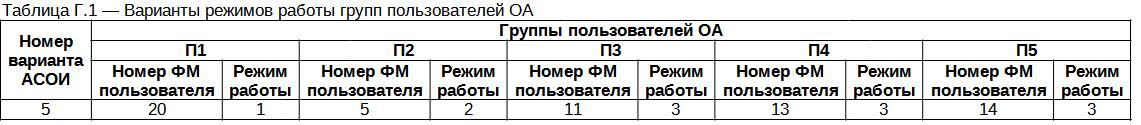
\includegraphics[width=14cm]
            {_docs/ТаблицаГ1ВариантыРежимовРаботыГруппПользователейОА.jpg}
        \caption{Варианты режимов работы групп пользователей ОА}
    \end{figure}

    При формировании табл.3.1 используются данные из табл.В.1 (количество пользователей по каж­дой группе)
    и табл. Г.1 (режим работы пользователей и ЭП). 

    \begin{figure}[h!]
        \centering
        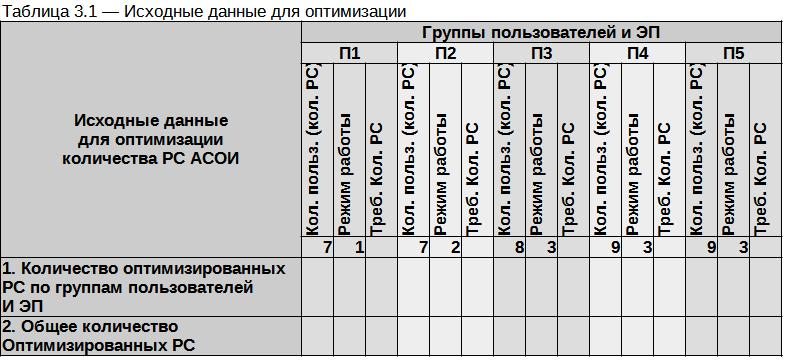
\includegraphics[width=14cm]
            {_docs/Таблица3-1ИсходныеДанныеДляОптимизации.jpg}
        \caption{Исходные данные для оптимизации}
    \end{figure}

    \newpage
    \textbf{Оптимизация (сокращение) количества РС АСОИ}.
    Она заключается в сокращении количества РС в рамках каждой группе пользователей и ЭП.
    Оптимизация включает выполнение следующих дей­ствий:
    \begin{enumerate}
        \item[1.] Определение для каждой группы требуемого количества РС для их нормального функционирова­ния.
        При этом используется анализ значения показателя режим сменности.
        Если режим сменности равен единице, то каждому пользователю (ЭП) необходима отдельная РС.
        При значении показателя два – два пользователя могут работать на одной станции.
        При значении показателя три – три пользователя. Пример приведен в табл. 3.2. 

        <<Треб. кол. РС>> = ОкруглениеВверх( <<Кол. польз. (кол. РС)>> / <<Режим работы>> )

        \textbf{Для П1:} $RoundUp(7 / 1) = 7$ 

        \textbf{Для П2:} $RoundUp(7 / 2) = 4$

        \textbf{Для П3:} $RoundUp(8 / 3) = 4$

        \textbf{Для П4:} $RoundUp(9 / 3) = 3$

        \textbf{Для П5:} $RoundUp(9 / 3) = 3$

        \item[2.] Определение для каждой группы <<Количество оптимизированных РС ...>> по формуле:   
        Количество оптимизированных РС по группе = Кол.РС - Треб.Кол.РС
        и заполнение полученными значениями строку <<Количество оптимизированных РС ...>> в табл. 3.2.

        <<Количество оптимизированных РС по группе>> = <<Кол. польз. (кол. РС)>> - <<Треб. кол. РС>>

        \textbf{Для П1:} $7 - 7 = 0$ 

        \textbf{Для П2:} $7 - 4 = 3$

        \textbf{Для П3:} $8 - 3 = 5$

        \textbf{Для П4:} $9 - 3 = 6$

        \textbf{Для П5:} $9 - 3 = 6$

        \item[3.] Определение <<Общее количество оптимизированных РС>> путем суммирования значений
        <<Коли­чество оптимизированных РС по группам>>. 

        $0 + 3 + 5 + 6 + 6 = 20$
    \end{enumerate}

    \begin{figure}[ht!]
        \centering
        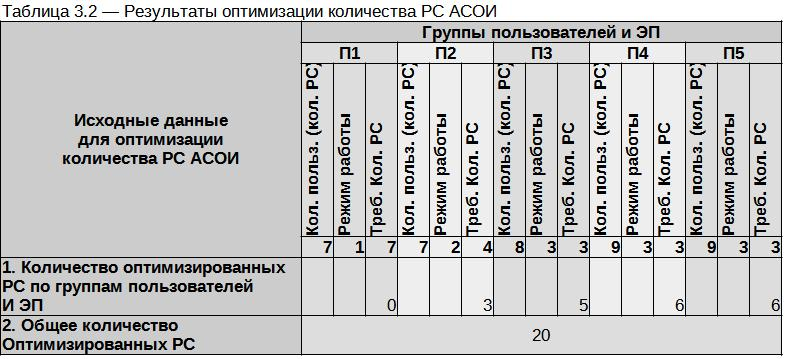
\includegraphics[width=14cm]
            {_docs/Таблица3-2РезультатыОптимизацииКоличестваРСАСОИ.jpg}
        \caption{Результаты оптимизации количества РС АСОИ}
    \end{figure}

    \paragraph{} \textbf{Размещение элементов АСОИ по помещениям}

    Цель размещения элементов АСОИ (пользователей, ЭП, СС и РС) - это расположение всех эле­ментов системы АСОИ
    по заданному варианту помещений ОА, при необходимо минимизировать пока­затели количество занимаемых помещений
    и их общей площади, выполняя при этом условия, ограни­чения и нормативы, перечисленные в п.2.
    
    Для представления исходных данных и результатов размещения предлагается табличный способ (см. табл.4.1).
    В таблице 4.1 представлены две группы объектов:

    1. «Элементы и группы элементов АСОИ» - графы с 1 по 7, которые описывают:

    \begin{itemize}
        \item[*] графа 1 – название групп элементов АСОИ (пользователи – П1, п2,..; ЭП – П6; серверов);
        \item[*] графа 2 – общее количество элементов в каждой из групп элементов АСОИ;
        \item[*] графа 3 – режим работы, используется только для пользователей и ЭП;
        \item[*] графа 4 – общее количество станций, необходимое для работы каждой группы элементов (по­сле оптимизации); 
        \item[*] графа 5 – номер станции, последовательно перечисляются все станции АСОИ;
        \item[*] графа 6 – список номеров рабочих мест (РМ), которые располагаются на определенных стан­циях;
        \item[*] графа 7 – минимально необходимая площадь для размещения элементов заданной группы элементов;
    \end{itemize}
    
    2. «Помещения ОА для размещения элементов  АСОИ» - графы с 8 по 9, которые описывают:
        
    \begin{itemize}
        \item[*] графа 8 – номер помещения из табл.Б.2  для размещения элементов АСОИ. 
        \item[*] графа 9 – общая площадь помещения из табл.Б.2. 
        \item[*] графа 10 – свободная площадь помещения после размещения элементов АСОИ. 
    \end{itemize}

    Процесс размещения элементов представляет последовательность следующих действий:
    \begin{enumerate}
        \item[1.] Формирование исходных данных путем заполнения таблицы 4.1 исходными данными.
        \item[2.] Размещение элементов АСОИ по помещениям ОА, при минимизации заданные показатели
        и вы­полняя предложенные условия, требования и нормативы. 
    \end{enumerate}

    Формирование исходными данными в виде табл. 4.1:
    \begin{itemize}
        \item[*] для каждой группы элементов формируется строка, в которой определяются графы 1 - 4, 7 (см. табл. 4.1);
        \item[*] для каждой группы элементов формируются графы «Номер станции»
        и «Список номеров РМ» (графы 5 и 6) и добавляются в виде строк в табл.4.1
        (фрагмент примера см. табл. 4.2) - отме­чены красным цветом.
    \end{itemize}

    \begin{figure}[ht!]
        \centering
        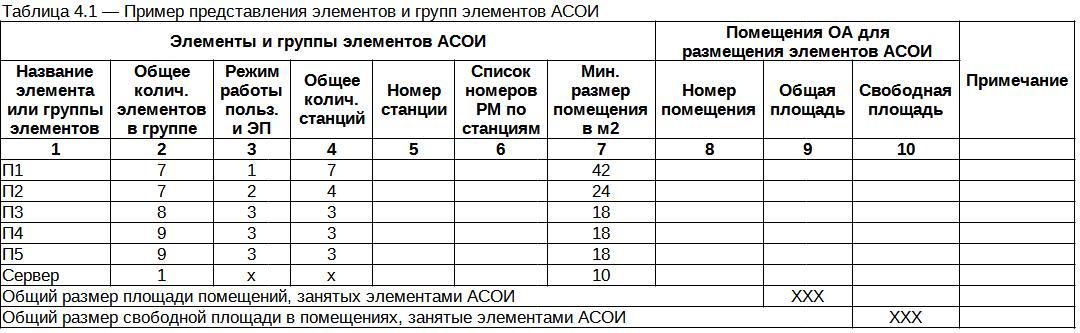
\includegraphics[width=14cm]
            {_docs/Таблица4-1ПримерПредставленияЭлементовИГруппЭлементовАСОИ.jpg}
        \caption{Пример представления элементов и групп элементов АСОИ}
    \end{figure}

    <<Минимальный размер помещения>> = <<Общее колич. станций>> * 6

    \textbf{Для П1:} $7 * 6 = 42$ 

    \textbf{Для П2:} $4 * 6 = 24$

    \textbf{Для П3:} $3 * 6 = 18$

    \textbf{Для П4:} $3 * 6 = 18$

    \textbf{Для П5:} $3 * 6 = 18$

    <<Минимальный размер сервера>> = 10

    \textbf{Для С1:} $10$

    \newpage
    \begin{figure}[ht!]
        \centering
        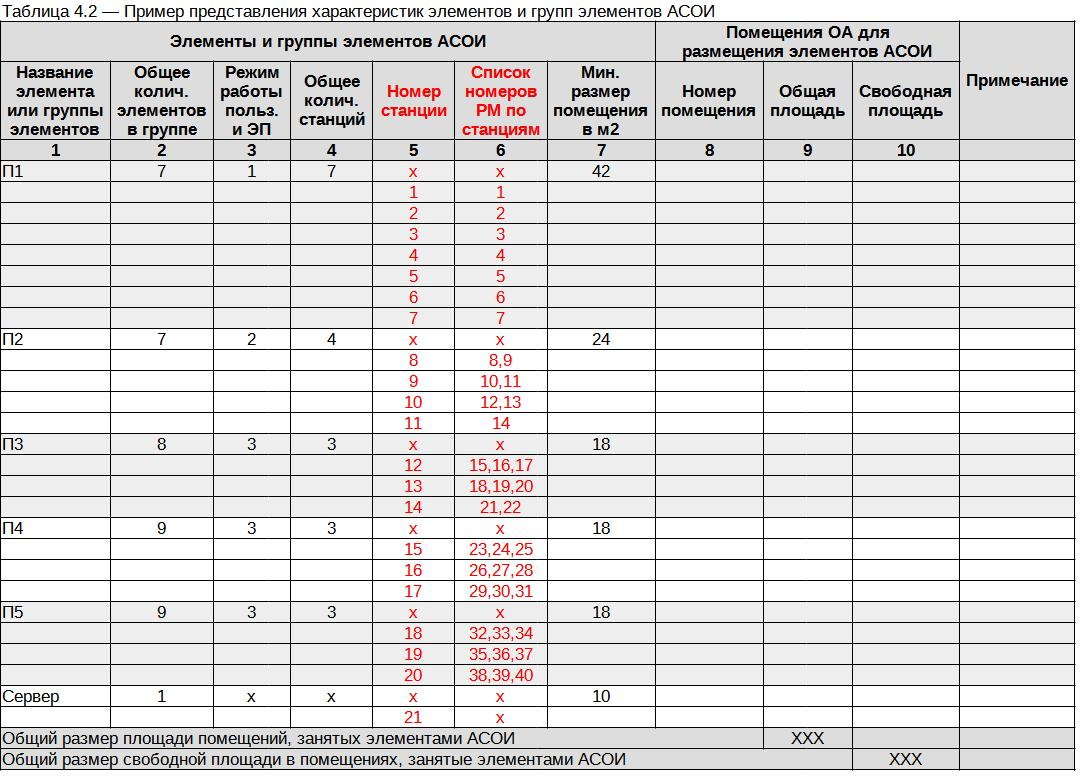
\includegraphics[width=14cm]
            {_docs/Таблица4-2ПримерПредставленияХарактеристикЭлементовИГруппЭлементовАСОИ.jpg}
        \caption{Пример представления характеристик элементов и групп элементов АСОИ}
    \end{figure}

    \textbf{Для П1:} Так как <<Общее колич. станций>> = 7, то получаем: 1,2,3,4,5,6,7.

    \textbf{Для П2:} Так как <<Общее колич. станций>> = 4, то получаем: 8,9,10,11.

    \textbf{Для П3:} Так как <<Общее колич. станций>> = 3, то получаем: 12,13,14.

    \textbf{Для П4:} Так как <<Общее колич. станций>> = 3, то получаем: 15,16,17.

    \textbf{Для П5:} Так как <<Общее колич. станций>> = 3, то получаем: 18,19,20.

    \textbf{Для C1:} 21

    \textbf{Для П1:} Так как <<Режим работы польз. и ЭП>> = 1 и <<Общее колич. станций>> = 7 и <<Общее колич. элементов в группе>> = 7
    то получаем: 1; и 2; и 3; и 4; и 5; и 6; и 7.

    \textbf{Для П2:} Так как <<Режим работы польз. и ЭП>> = 2 и <<Общее колич. станций>> = 4 и <<Общее колич. элементов в группе>> = 7
    то получаем: 8,9; и 10,11; и 12,13; и 14.

    \textbf{Для П3:} Так как <<Режим работы польз. и ЭП>> = 3 и <<Общее колич. станций>> = 3 и <<Общее колич. элементов в группе>> = 8
    то получаем: 15,16,17; и 18,19,20; и 21,22.

    \textbf{Для П4:} Так как <<Режим работы польз. и ЭП>> = 3 и <<Общее колич. станций>> = 3 и <<Общее колич. элементов в группе>> = 9
    то получаем: 23,24,25; и 26,27,28; и 29,30,31.

    \textbf{Для П5:} Так как <<Режим работы польз. и ЭП>> = 3 и <<Общее колич. станций>> = 3 и <<Общее колич. элементов в группе>> = 9
    то получаем: 32,33,34; и 35,36,37; и 38,39,40.

    \textbf{Для C1:} x

    \newpage

    Размещение элементов АСОИ по помещениям.
    Выполняется самостоятельно.
    Возможны два способа реализации размещения элементов:

    \begin{enumerate}
        \item[1.] «Подбор» возможного варианта размещения всех элементов АСОИ без учета показателей мини­мизации.
        Рассматривается далее.
        \item[2.] Применение одного из методов оптимизации... . 
    \end{enumerate}

    При размещении элементов целесообразно использовать табл. 4.3. и следующие рекомендации:
    \begin{enumerate}
        \item[1.] Для представления результатов размещения элементов использовать таблицу 4.3,
        которая явля­ется расширением табл. 4.2 (дополняются строки по помещениям).
        \item[2.] Информацию об отдельном помещении, которое использовано для размещения определенной группы элементов
        представлять в таблице 4.3 в виде отдельной строки с заполненными гра­фами с 8 по 10
        (на рис. 4.3 эти результаты изображены синим цветом). 
        \item[3.] Под строкой, описывающей использованное помещение, рекомендуется располагать строки,
        пред­ставляющие описание станций и список РМ, располагаемых в этих помещениях.
        \item[4.] Если для размещения группы элементов используется более одного помещения
        (см. группа П2, табл.4.3), то информация о соответствующих помещениях добавляется в таблицу. 
    \end{enumerate}

    Пример фрагмента размещения пользователей, ЭП и элементов АС (сервера),
    а также ре­зультаты расчета итоговых показателей приведены в табл. 4.3.

    По результатам решения задачи формируются следующие результаты:
    \begin{enumerate}
        \item[1.] Результаты размещения элементов в виде таблицы 4.3.
        \item[2.] Расчет итоговых показателей: общее количество помещений,
        общее количество занятых помеще­ний, общий размер площади помещений,
        общий размер занятых помещений, общий объем свободной площади в занятых помещениях.
        \item[3.] При использовании первого способа решения – приводится описание способ и результатов реше­ния задачи.
    \end{enumerate}

    \newpage

    \textbf{Для П1:} 42 м2 <= 25 м2 (помещение 8) + 25 м2 (помещение 9)

    \textbf{Для П2:} 24 м2 <= 25 м2 (помещение 4)

    \textbf{Для П3:} 18 м2 <= 20 м2 (помещение 2)

    \textbf{Для П4:} 18 м2 <= 20 м2 (помещение 3)

    \textbf{Для П5:} 18 м2 <= 20 м2 (помещение 5)

    \textbf{Для C1:} 10 м2 <= 10 м2 (помещение 1)

    \begin{figure}[ht!]
        \centering
        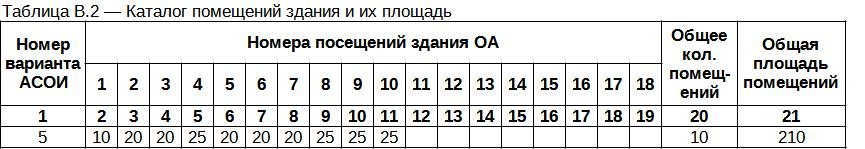
\includegraphics[width=14cm]
            {_docs/ТаблицаВ2КаталогПомещенийЗданияИИхПлощадь.jpg}
        \caption{Каталог помещений здания и их площадь}
    \end{figure}

    <<Свободная площадь>> = <<Общая площадь>> - 6 * <<Количество станций>>

    \textbf{Для П1:} 25 - 6 * 4 = 1. 25 - 6 * 3 = 7.

    \textbf{Для П2:} 25 - 6 * 4 = 1

    \textbf{Для П3:} 20 - 6 * 3 = 2

    \textbf{Для П4:} 20 - 6 * 3 = 2

    \textbf{Для П5:} 20 - 6 * 3 = 2

    <<Свободная площадь>> = <<Общая площадь>> - 10 * <<Количество станций>>

    \textbf{Для C1:} 10 - 10 * 1 = 0

    \begin{figure}[ht!]
        \centering
        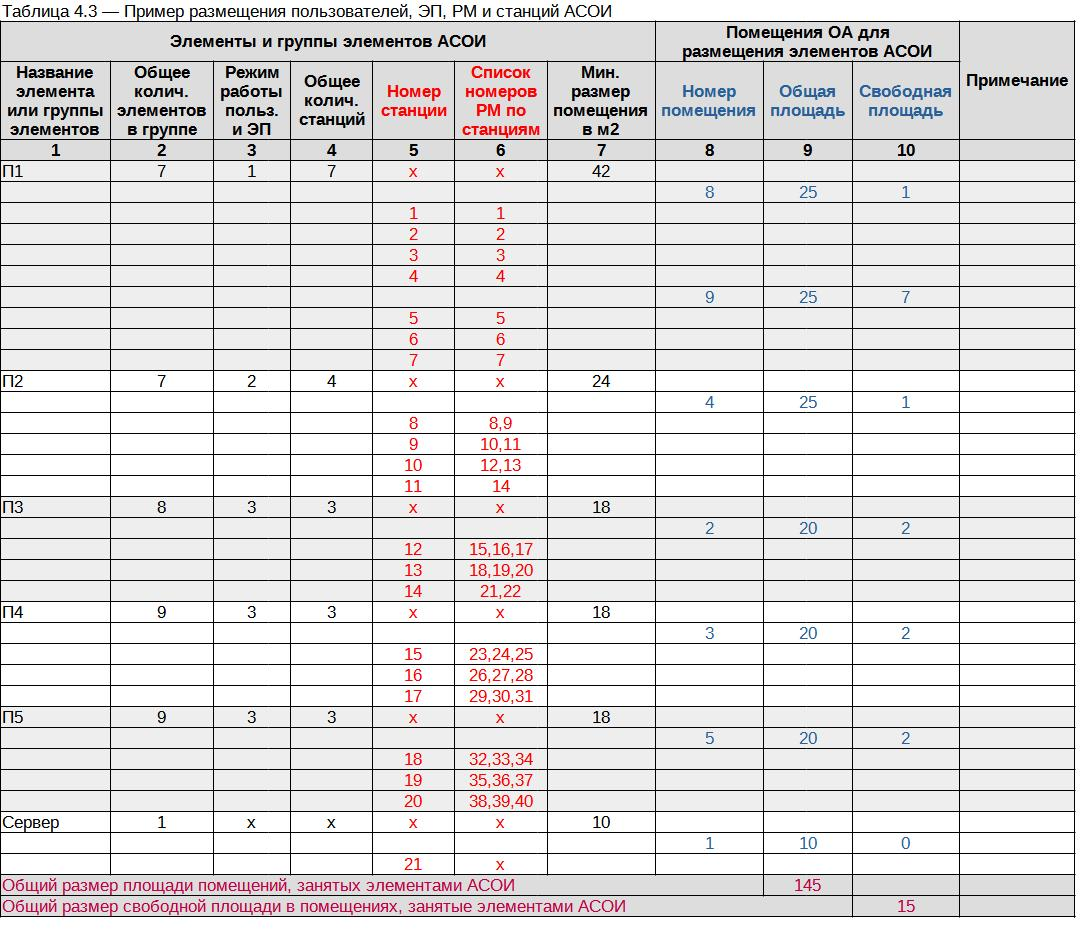
\includegraphics[width=14cm]
            {_docs/Таблица4-3ПримерРазмещенияПользователейЭПРМИСтанцийАСОИ.jpg}
        \caption{Пример размещения пользователей, ЭП, РМ И станций АСОИ}
    \end{figure}

    \newpage

    За все компы отдаём другую цену (их количество уменьшилось). Несколько пользователей на комп.

    За принтеры отдаём другую цену (количество компов уменьшилось, а следовательно количество принтеров уменьшилось).

    \begin{figure}[!hp]
        \centering
        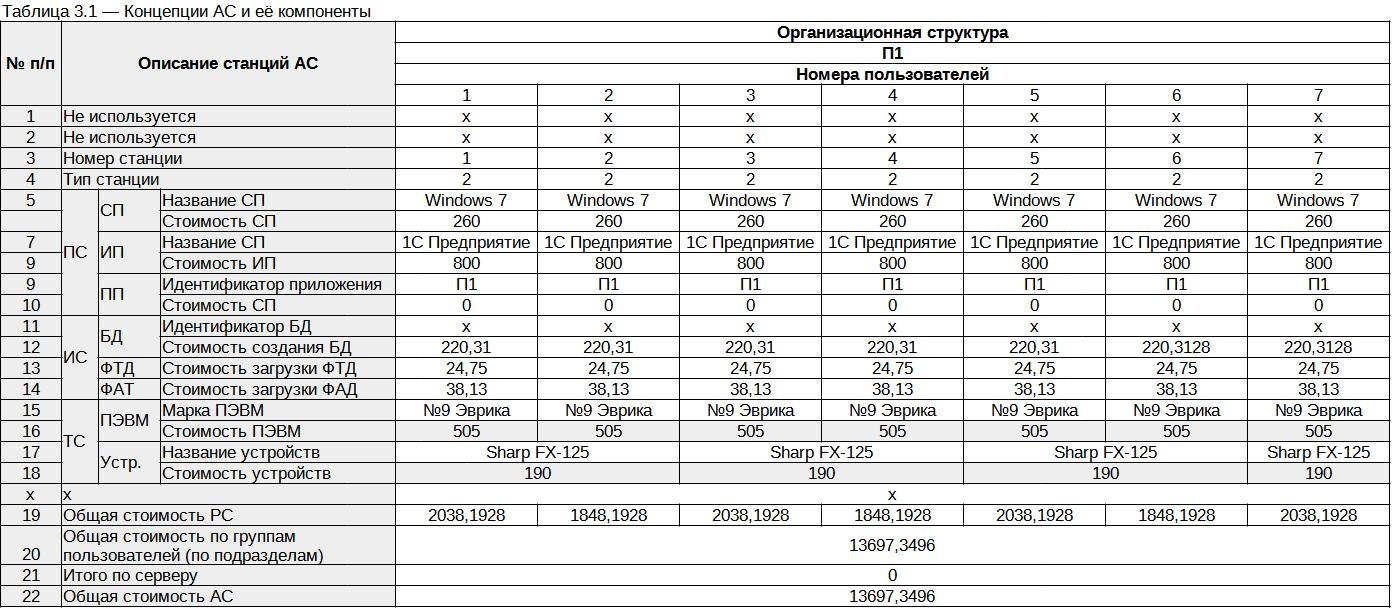
\includegraphics[height=6cm]
            {_docs/Таблица3-1КонцепцияАСИЕеКомпоненты__лаб2_П1.jpg}
        \caption{Концепция АС и её компоненты}
    \end{figure}

    \begin{figure}[!hp]
        \centering
        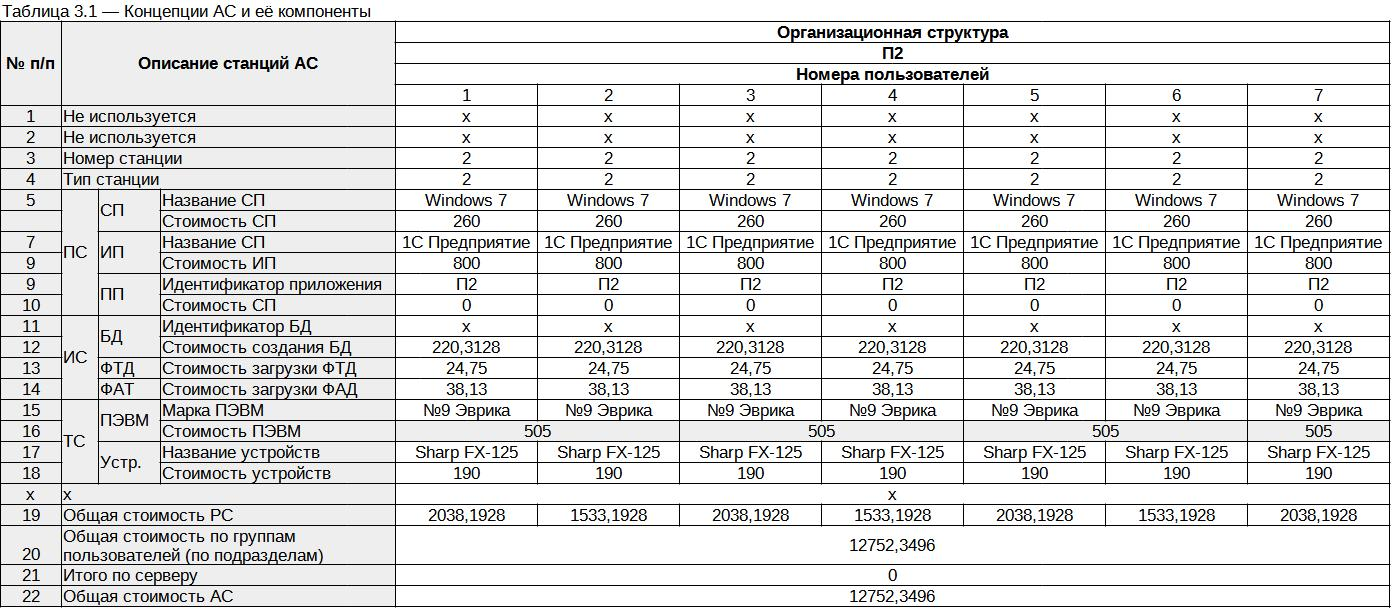
\includegraphics[height=6cm]
            {_docs/Таблица3-1КонцепцияАСИЕеКомпоненты__лаб2_П2.jpg}
        \caption{Концепция АС и её компоненты}
    \end{figure}

    \begin{figure}[!hp]
        \centering
        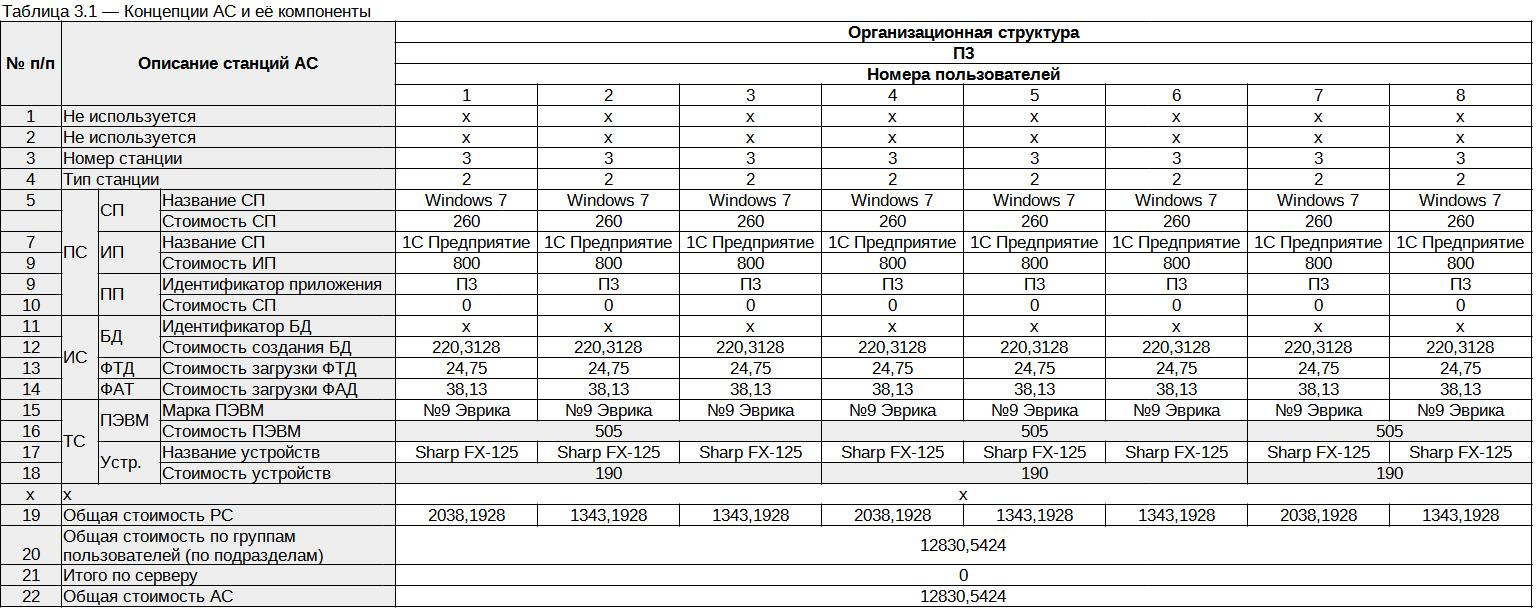
\includegraphics[height=6cm]
            {_docs/Таблица3-1КонцепцияАСИЕеКомпоненты__лаб2_П3.jpg}
        \caption{Концепция АС и её компоненты}
    \end{figure}

    \begin{figure}[!hp]
        \centering
        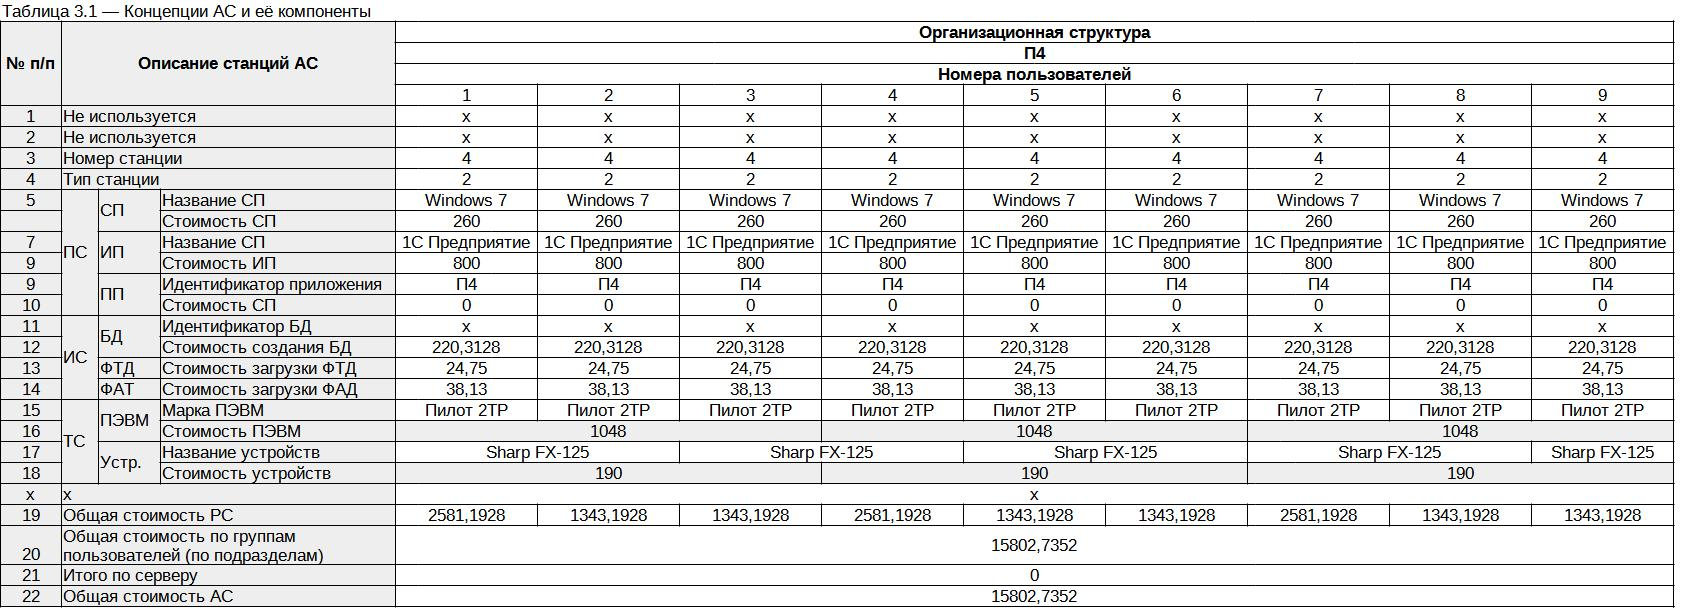
\includegraphics[height=6cm]
            {_docs/Таблица3-1КонцепцияАСИЕеКомпоненты__лаб2_П4.jpg}
        \caption{Концепция АС и её компоненты}
    \end{figure}

    \begin{figure}[!hp]
        \centering
        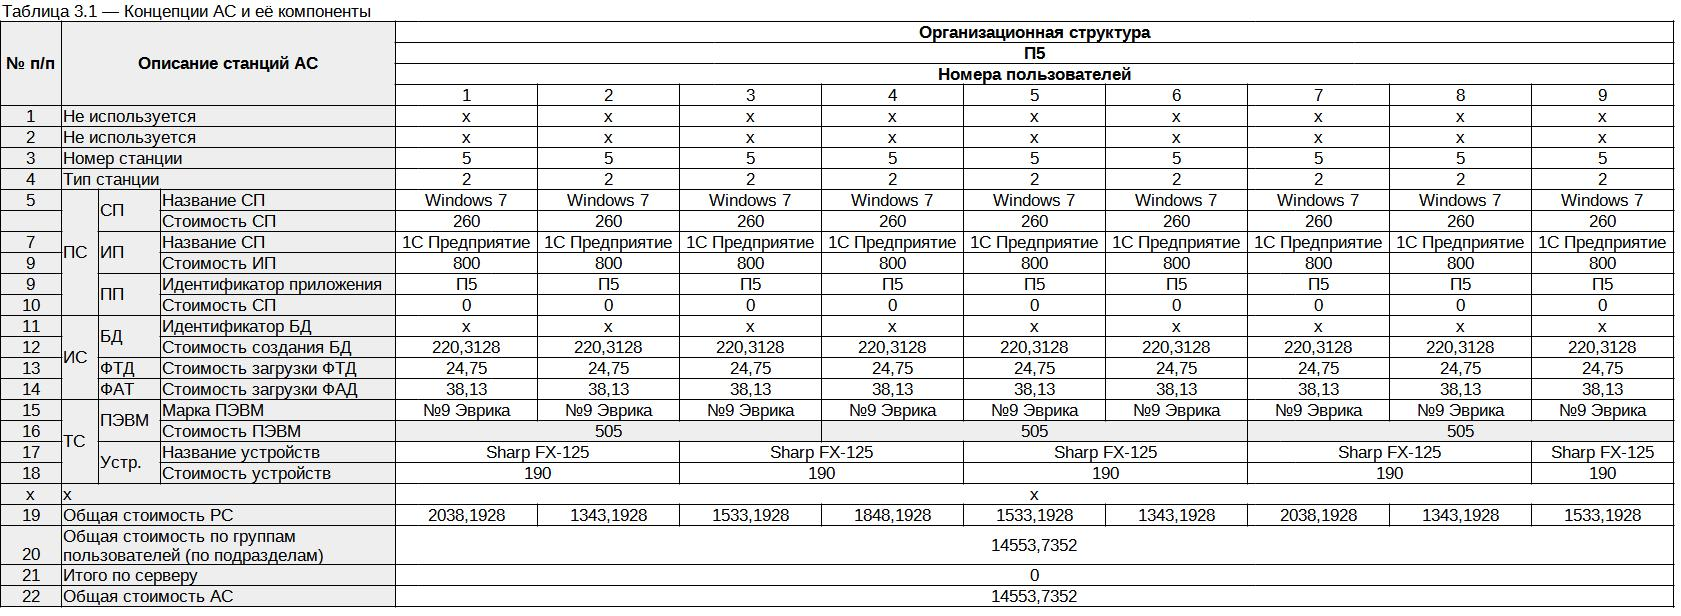
\includegraphics[height=6cm]
            {_docs/Таблица3-1КонцепцияАСИЕеКомпоненты__лаб2_П5.jpg}
        \caption{Концепция АС и её компоненты}
    \end{figure}

    % \begin{figure}[!hp]
    %     \centering
    %     \includegraphics[height=6cm]
    %         {_docs/Таблица3-1КонцепцияАСИЕеКомпонентыСС1.jpg}
    %     \caption{Концепция АС и её компоненты}
    % \end{figure}

    \begin{figure}[!hp]
        \begin{minipage}{0.48\textwidth}
            \centering
            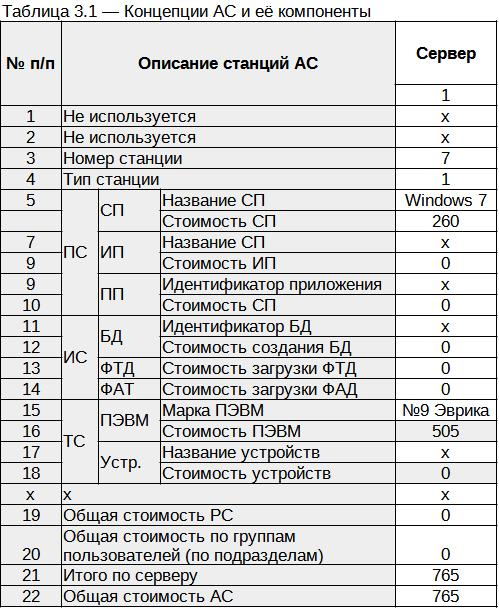
\includegraphics[height=8cm]
            {_docs/Таблица3-1КонцепцияАСИЕеКомпоненты__лаб2_С1.jpg}
            \caption{Концепция АС и её компоненты}
        \end{minipage}
        \begin{minipage}{0.48\textwidth}
            \centering
            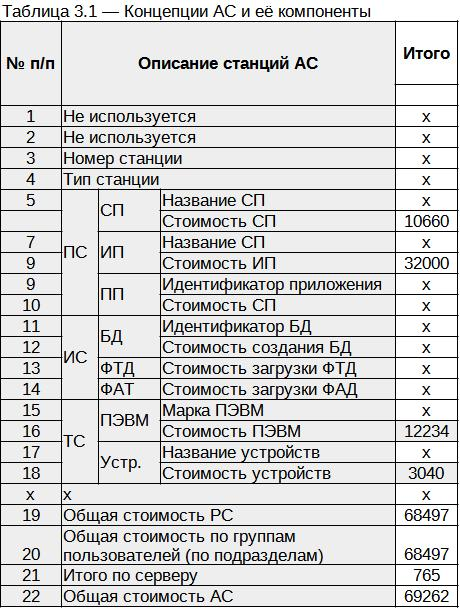
\includegraphics[height=8cm]
            {_docs/Таблица3-1КонцепцияАСИЕеКомпоненты__лаб2.jpg}
            \caption{Концепция АС и её компоненты}
        \end{minipage}
     \end{figure}

    \begin{figure}[h!]
        \centering
        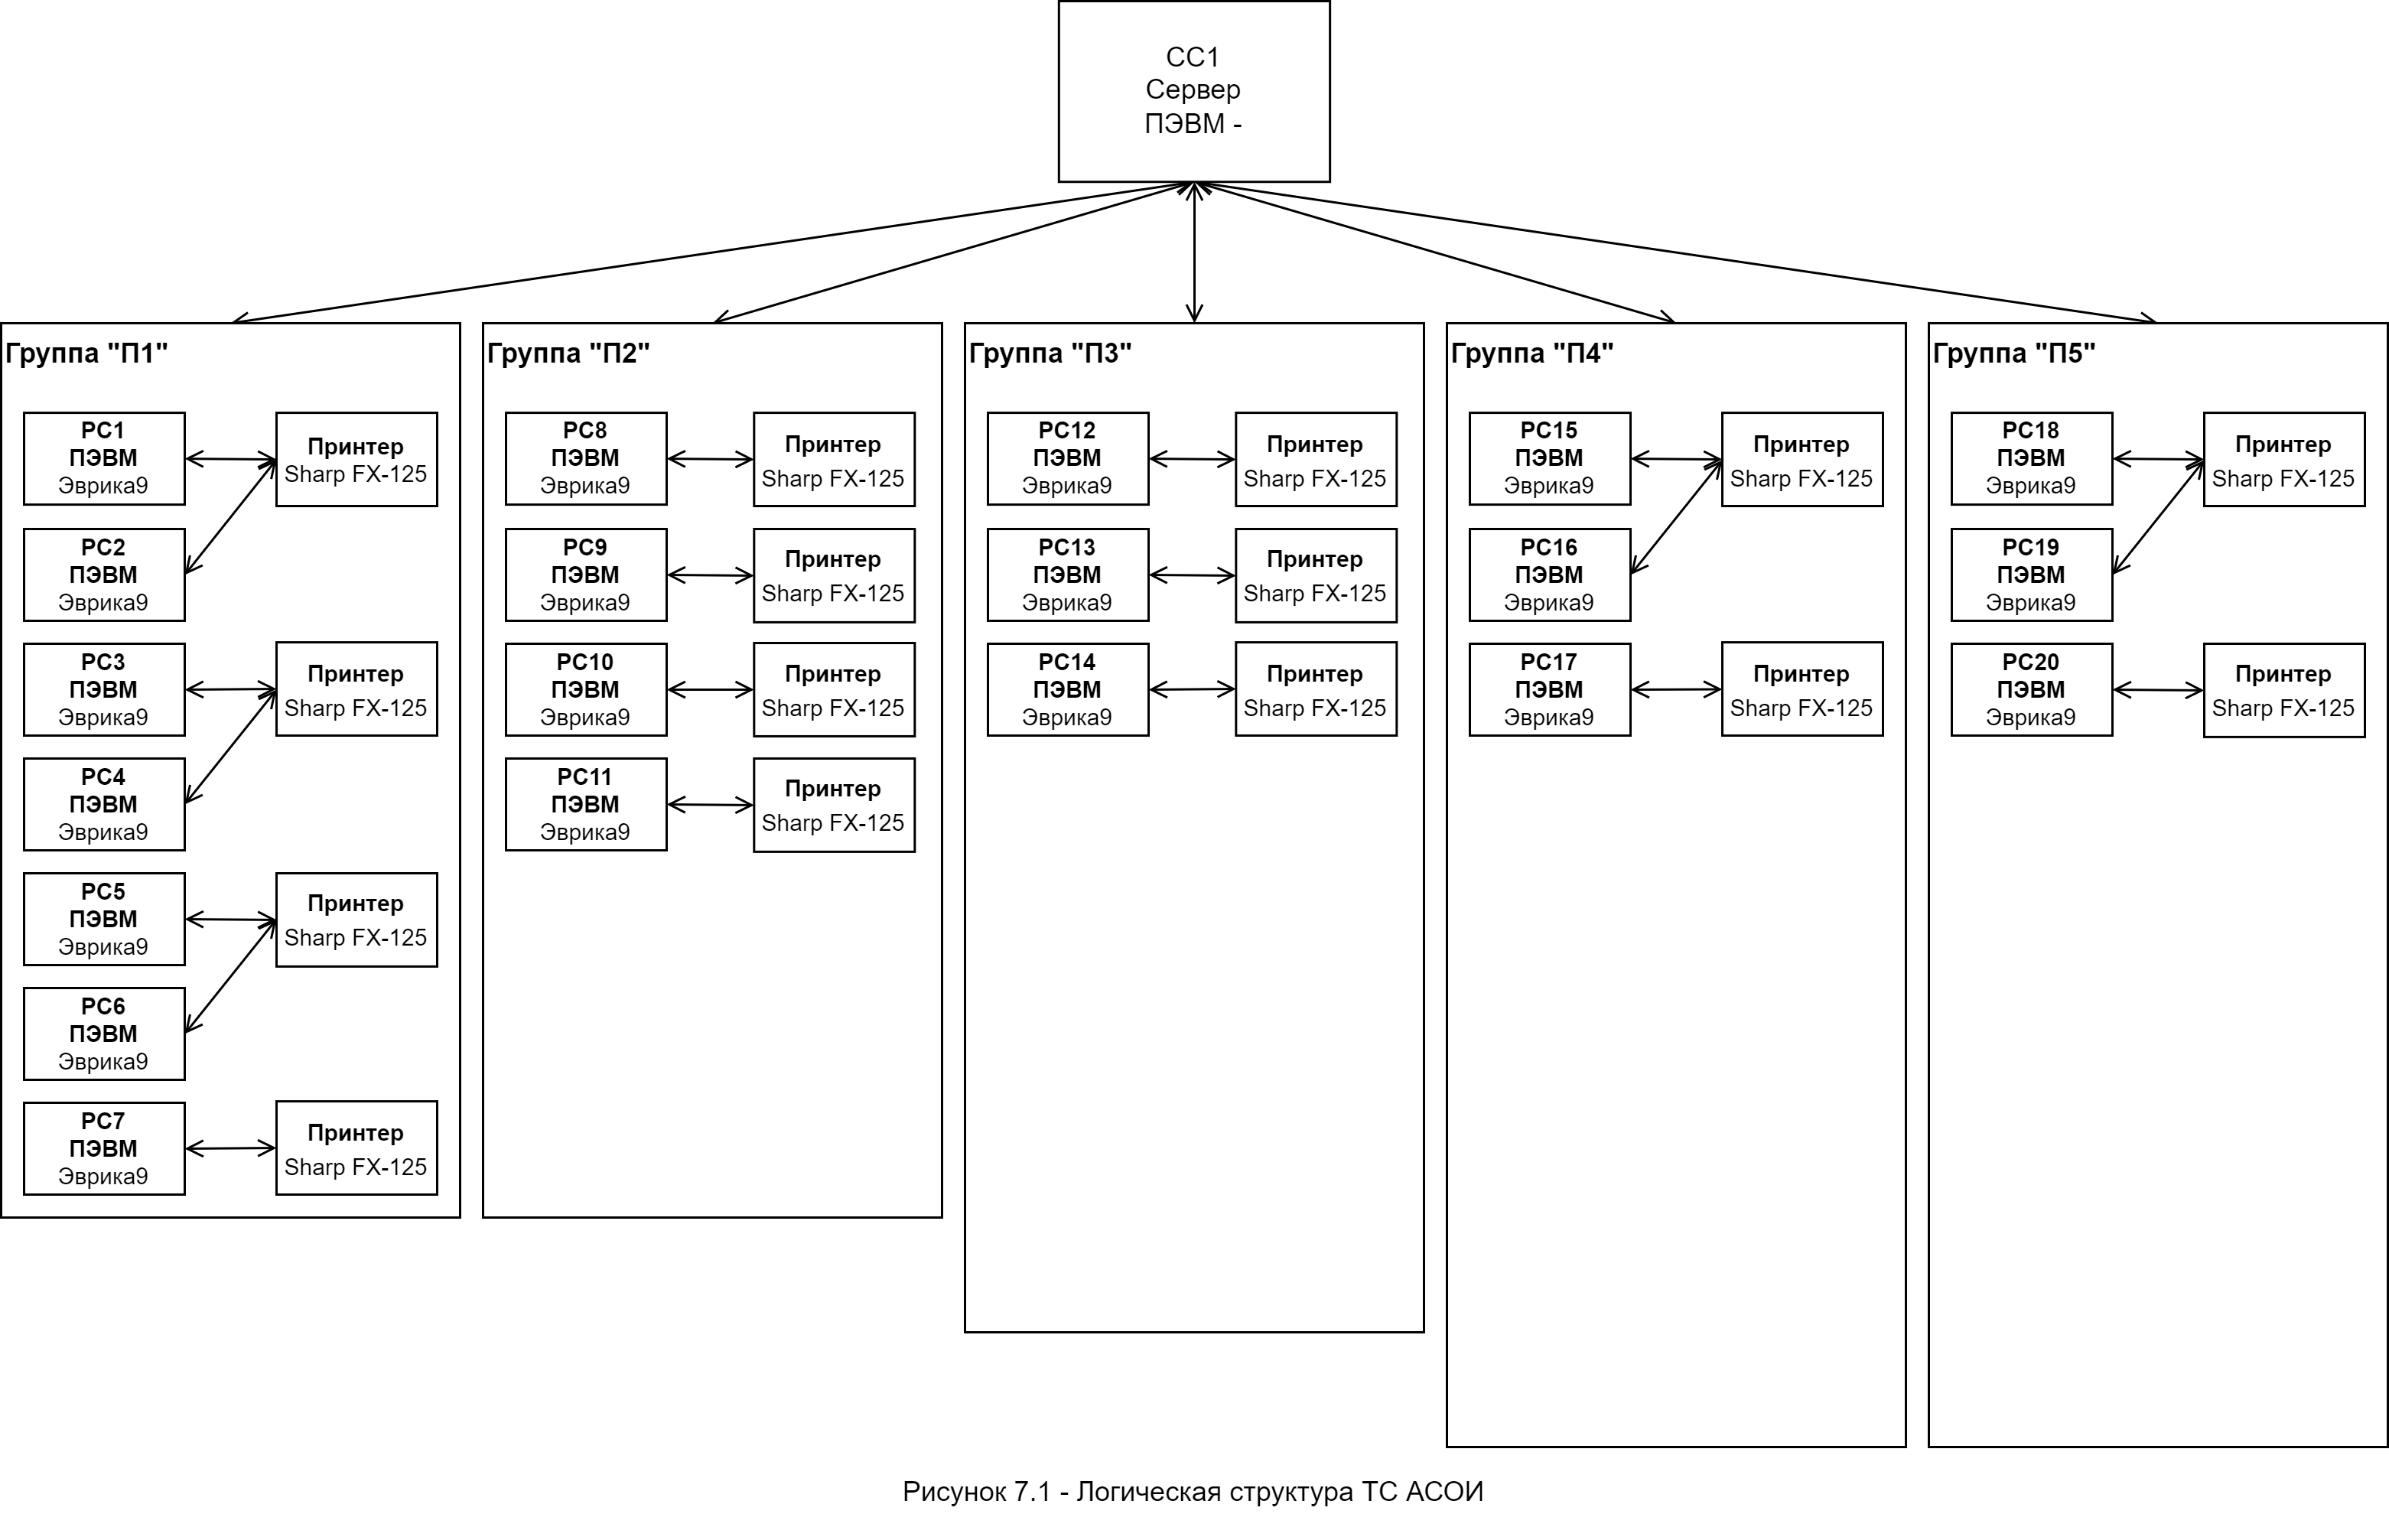
\includegraphics[width=16cm]
            {_docs/Рисунок7-1ЛогическаяСтруктураТСАСОИ__лаб2.png}
        \caption{Логическая структура ТС АСОИ}
    \end{figure}
\end{document}
